\documentclass[10pt,sigconf,nonacm]{acmart}

\settopmatter{printacmref=false, printccs=false, printfolios=true}

\usepackage{booktabs}

\graphicspath{{./}{../compare/results/}{figure/}{figures/}}

\setcopyright{none}
\acmDOI{}
\acmISBN{}
\acmConference[COMS E6868]{Embedded Scalable Platforms}{Spring 2025}{Columbia University}
\acmYear{2025}
\copyrightyear{2025}

\begin{document}
\title{System-Level Modeling of Multi-Accelerator Architectures via Analytical Cost Model Integration}
\subtitle{\normalsize COMS E6868 - Embedded Scalable Platforms - Spring 2026}

\author{Kevin Liu}
\email{kl3755@columbia.edu}

\renewcommand{\shortauthors}{K. Liu}

\begin{abstract}
Modern deep learning workloads run on platforms with multiple accelerators connected by a Network-on-Chip (NoC) and shared DRAM. Analytical cost models such as MAESTRO and Timeloop estimate performance for a single accelerator but do not capture system-level effects (inter-accelerator communication, DRAM contention). This project proposes a system-level modeling framework that integrates these accelerator-level models with explicit NoC and memory modeling. At midterm we have (1) implemented output-stationary (ShiDianNao), weight-stationary (NVDLA), and row-stationary (Eyeriss) dataflows in both MAESTRO and Timeloop on the same conv layer (107M MACs) and 256-PE setup, (2) established a reproducible pipeline (Docker, parsing, comparison plots), and (3) compared latency, energy, and EDP across frameworks. Next we will design the system-level framework and integrate NoC/DRAM modeling, then simulate representative DNN workloads on multi-accelerator systems.
\end{abstract}

\maketitle

\section{Introduction}
\label{sec:intro}

This report summarizes progress on the project proposed at the start of the semester. The goal is to build a \emph{system-level} modeling framework that reuses analytical accelerator cost models (MAESTRO, Timeloop) and adds explicit modeling of NoC and shared DRAM so that multi-accelerator systems can be evaluated without cycle-accurate simulation.

\subsection{Motivation}
Different kinds of accelerators are good at different dataflows (e.g., output-stationary vs.\ weight-stationary vs.\ row-stationary), but building a real accelerator is time-consuming and costly. It is important to model performance before committing to hardware. Analytical models such as MAESTRO~\cite{maestro2019micro} and Timeloop~\cite{timeloop2019ispass} are effective for exploring dataflows and mappings on a single accelerator. They do not, however, model performance degradation from NoC congestion or DRAM contention when multiple accelerators run concurrently. System-level frameworks like SCAR~\cite{scar2024micro} and MAGMA~\cite{magma2022hpca} address scheduling and mapping across multiple cores but use their own performance estimators. This project unifies accelerator-level models (MAESTRO, Timeloop) with system-level NoC/DRAM modeling so that we can plug in established cost models and still capture system effects.

\section{Progress and Experimental Setup}
\label{sec:progress}

\subsection{Accelerator-Level Comparison (Milestones 2 \& 3)}

We implemented the three representative dataflows---output-stationary (OS, ShiDianNao), weight-stationary (WS, NVDLA), and row-stationary (RS, Eyeriss)---in both MAESTRO and Timeloop and compared their predicted performance on the \emph{same} conv layer.

\textbf{Workload.} One 2D conv layer: batch $N=1$, input/output channels $C=M=64$, filter $R=S=3$, output spatial $P=Q=56$. Total MACs $= N \cdot M \cdot C \cdot R \cdot S \cdot P \cdot Q = 107{,}495{,}424$ (107M).

\textbf{Accelerator size.} 256 PEs in both tools: MAESTRO via \texttt{num\_pes: 256} in the HW file; Timeloop via a 2-level arch (1-PE) run with latency scaled by $1/256$ to obtain a 256-PE equivalent for fair comparison.

\textbf{MAESTRO.} Hardware described in a \texttt{.m} file (PE count, L1/L2 size constraints, NoC and off-chip bandwidth). Dataflow in separate mapping files (TemporalMap, SpatialMap, Cluster over dimensions $K,C,R,S,Y,X$). We run OS, WS, RS mappings and parse stdout for runtime (cycles) and total energy (in ``MAC energy'' units). Energy is converted to $\mu$J using $0.21$ pJ/MAC.

\textbf{Timeloop.} Architecture and mapping in YAML: hierarchy (MainMemory $\to$ Buffer $\to$ MACC), technology, global\_cycle\_seconds, and (for a 256-PE variant) spatial mesh. We use the v0.4 front-end and run \texttt{timeloop model} for OS, WS, RS with the same problem and 2-level arch inside Docker (timeloopaccelergy/timeloop-accelergy-pytorch). Stats (cycles, energy in $\mu$J, utilization) are parsed into CSV and merged with MAESTRO for plots.

\textbf{Metrics.} We compare latency (cycles), energy ($\mu$J), and EDP (cycles $\times$ $\mu$J). Because the two tools use different cycle and energy models, raw latency and energy can differ; EDP is used as the main cross-framework metric. Plots are generated for latency-by-dataflow, energy-by-dataflow, and EDP, with fixed Y-axis scales for readability. Figure~\ref{fig:latency_energy} shows latency and energy by dataflow; Figure~\ref{fig:edp} shows EDP.

\begin{figure}[t]
  \centering
  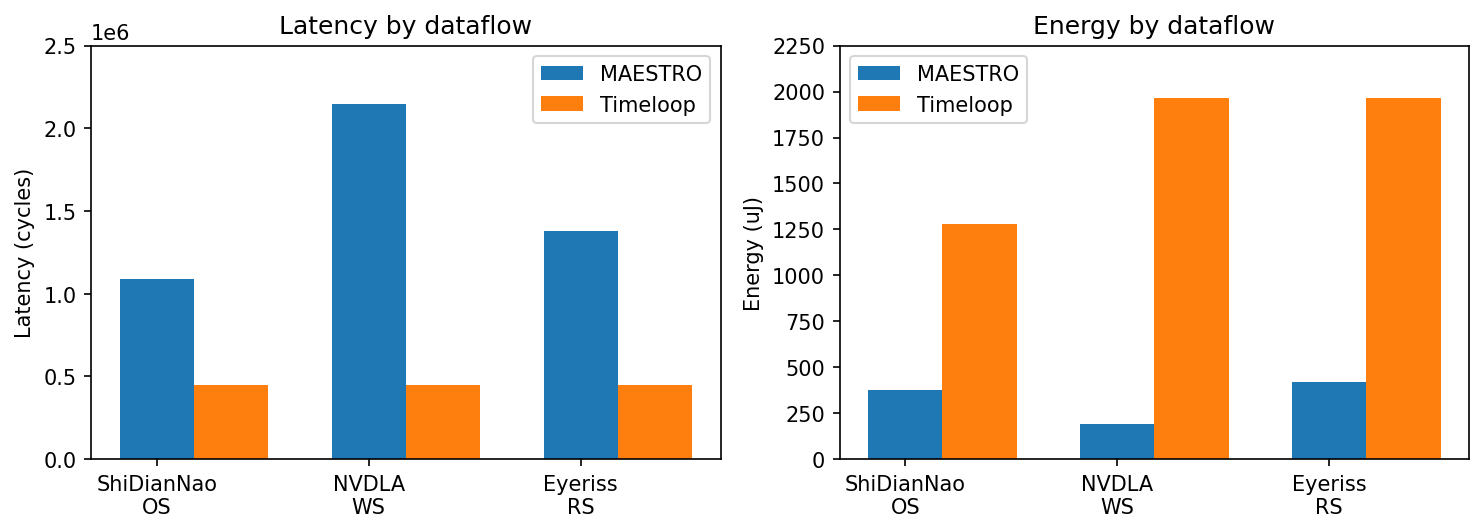
\includegraphics[width=\columnwidth]{comparison_latency_energy.png}
  \caption{Latency (cycles) and energy ($\mu$J) by dataflow for MAESTRO and Timeloop on the same 107M-MAC layer (256-PE equivalent).}
  \label{fig:latency_energy}
\end{figure}

\begin{figure}[t]
  \centering
  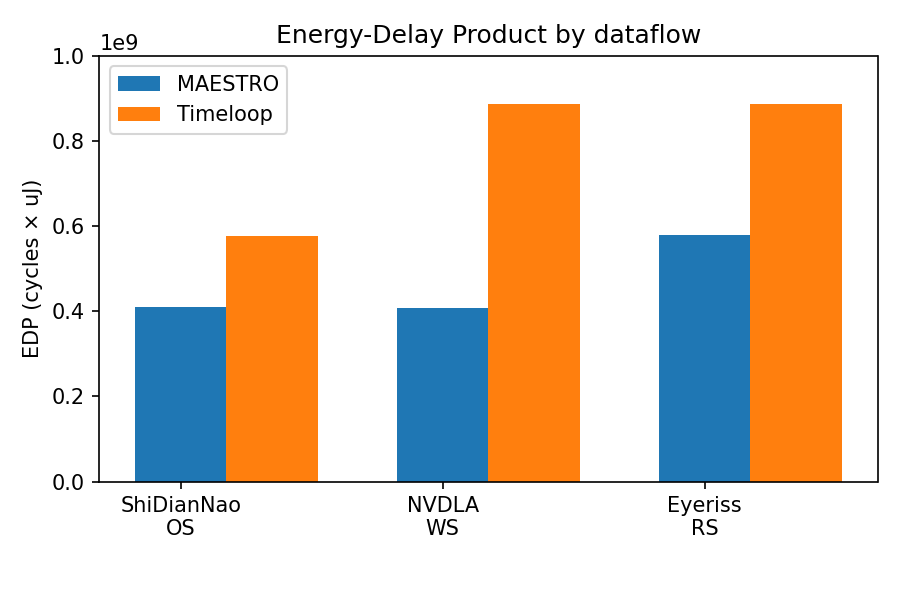
\includegraphics[width=\columnwidth]{comparison_edp.png}
  \caption{Energy-Delay Product by dataflow. EDP is used as the main cross-framework comparison metric.}
  \label{fig:edp}
\end{figure}

\subsection{Reproducibility}

The pipeline is automated: (1)./compare/timeloop/run\_timeloop.sh runs Timeloop OS/WS/RS in Docker and writes timeloop.stats.txt into compare/results/; (2) parse\_timeloop.py and parse\_maestro.py produce results\_timeloop.csv and results\_maestro.csv; (3) plot\_results.py merges them, applies 256-PE scaling for Timeloop, and outputs summary\_table.csv and comparison PNGs.

\section{Validation Plan}
\label{sec:validation}

\textbf{Accelerator-level (current).} Consistency between MAESTRO and Timeloop is assessed by (1) using the same layer and same effective PE count, (2) comparing EDP and relative ranking of dataflows (OS vs WS vs RS), and (3) documenting differences in cycle and energy models (see project \texttt{TASKS\_GUIDE.md} and midterm slides).

\textbf{System-level (next).} After integrating NoC and DRAM models, we will (1) compare predicted latency and scalability trends with published system-level approaches (e.g., MAGMA, SCAR) where possible; (2) vary the number of accelerator instances and NoC/DRAM bandwidth and report sensitivity; (3) run representative DNN workloads (e.g., a subset of layers from a small CNN) on a multi-accelerator configuration and report end-to-end latency. The goal is trend accuracy for design-space exploration, not cycle-level agreement.

\section{Next Steps}
\label{sec:next}

\begin{enumerate}
  \item \textbf{Design the system-level framework} (by Mar.\ 23): Define the abstraction that takes per-accelerator costs (from MAESTRO/Timeloop) and combines them with NoC and DRAM models.
  \item \textbf{Integrate inter-accelerator communication and DRAM modeling} (by Mar.\ 31): Add analytical or simplified models of NoC traversal and shared DRAM bandwidth allocation.
  \item \textbf{Simulation of representative DNN workloads} (by Apr.\ 15): Run one or more small DNNs (or layer subsets) on a multi-accelerator system in the framework and report latency and scalability.
  \item \textbf{System-level optimization} (by May 4): Explore mapping and scheduling strategies inspired by MAGMA and SCAR.
  \item \textbf{Final report and presentation} (May 14).
\end{enumerate}

\section{Milestones}
\label{sec:milestones}

Literature review (Feb.\ 18); implement OS/WS/RS in MAESTRO and Timeloop and compare (Feb.\ 25); study dataflow semantics (Mar.\ 4); design system-level framework (Mar.\ 10); integrate NoC/DRAM (Mar.\ 31); simulate DNN workloads on multi-accelerator systems (Apr.\ 15); system-level optimization (May 4); final analysis and report (May 6); final presentation and report (May 14).

\bibliographystyle{unsrt}
\bibliography{ref}

\end{document}
